\subsection{Data Preparation}\label{sec:DP}
\begin{tcolorbox}[title=Data Validation]
\textbf{Martin Kerdaniel:} Data is messy, Alison.  \\ 
\textbf{Alison MacIntosh:} Even when it's been cleaned?  \\ 
\textbf{Martin Kerdaniel:} Especially when it's been cleaned.\\[-0.6cm]
\begin{flushright}
-- P. Boily, I. Kiewiet, \textit{The Great Balancing Act}.
\end{flushright}
\end{tcolorbox}
\noindent
Once the raw data has been collected and stored in a dataset that is accessible to the quantitative consultants, the focus should shift to data cleaning and processing.  This requires testing for \textbf{soundness} and fixing \textbf{errors}, designing and implementing strategies to deal with \textbf{missing values} and \textbf{outlying/influential observations}, as well as low-level \textbf{exploratory data analysis} and \textbf{visualisation} to determine what \textbf{data transformations} and \textbf{dimension reduction} approaches will be needed in the final analysis. Consultants should be prepared to spend up to 80\% of their time processing and cleaning the data.  
\newl 
The following remarks must be taken to heart during this stage: 
\begin{itemize}[noitemsep]
\item Processing should \textbf{NEVER} be done on the original dataset -- make copies along the way.
\item {\textbf{ALL}} cleaning steps and procedures need to be documented.
\item If \textbf{too much} of the data requires cleaning up, the data collection procedure might need to be \textbf{revisited}.
\item An entire record should only be discarded as a \textbf{last resort}.
\end{itemize}
Another thing to keep in mind is that cleaning and processing may need to take place more than once depending on the type of data collection (one pass, batch, continuously). \par Finally, note that we are assuming that the datasets of interest contain only numerical and/or categorical observations. Additional steps must be taken when dealing with unstructured data, such as text or images.  

\subsubsection{General Principles}
\begin{tcolorbox}[title=Data Validation]
\textbf{Dilbert:} I didn't have any accurate numbers, so I just made up this one. Studies have shown that accurate numbers aren't any more useful that the ones you make up. \\ 
\textbf{Pointy-Haired Boss:} How many studies showed that? \\ 
\textbf{Dilbert:} [\textit{beat}] Eighty-seven.\\[-0.6cm]
\begin{flushright}
-- Scott Adams, \newhref{http://dilbert.com/strip/2008-05-08}{Dilbert}, 8 May 2008
\end{flushright}
\end{tcolorbox}
\noindent
\paragraph{Approaches to Data Cleaning}
There are two main \textbf{philosophical} approaches to data cleaning and validation, which we call
\begin{itemize}[noitemsep]
\item methodical, and 
\item narrative.
\end{itemize}
\newpage\noindent The \textbf{methodical} approach consists in running through a \textbf{check list} of potential issues and flagging those that apply to the data.
The \textbf{narrative} approach, on the other hand, consists in \textbf{exploring} the dataset while searching for unlikely or irregular patterns. Which approach the consultant opts to follow depends on a number of factors, not least of which is the client's needs and views  on the matter -- consultants have a responsibility to discuss this point with the clients.
\begin{table}[t]
\centering
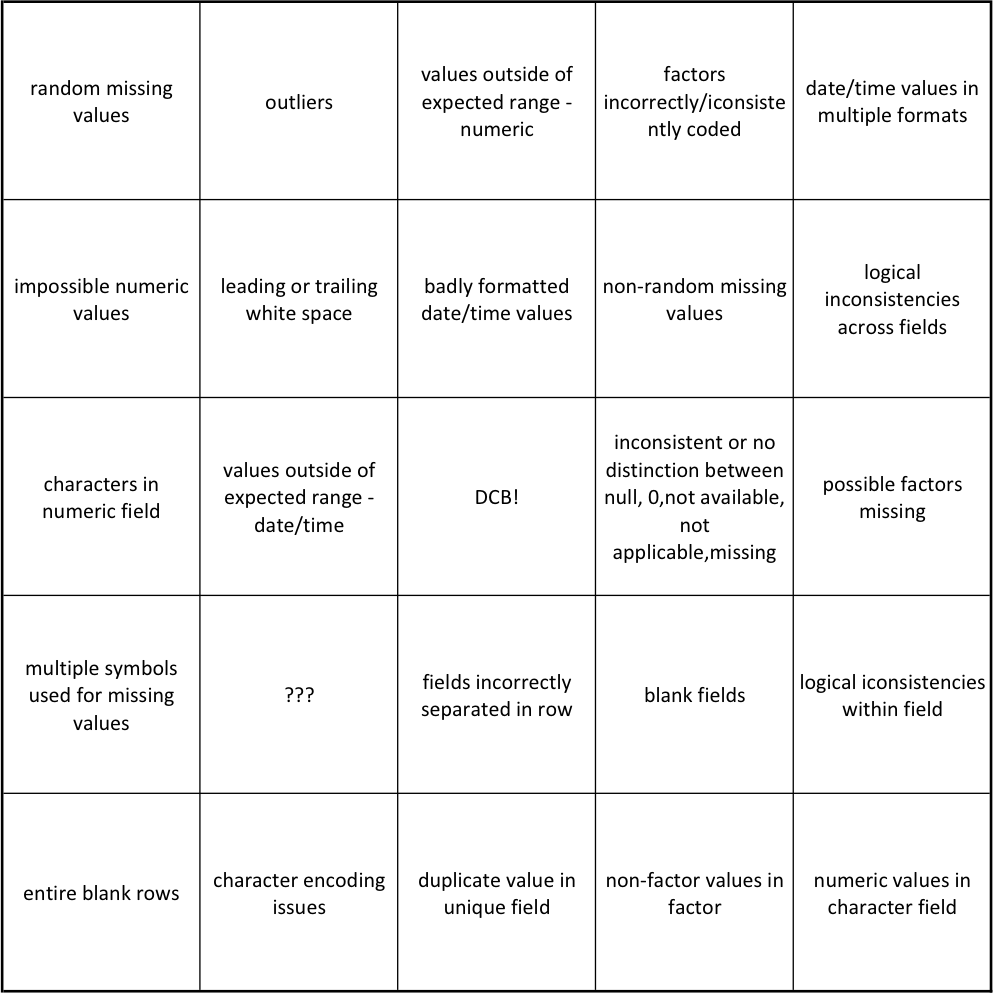
\includegraphics[width=\textwidth]{images/DP/bingo.png}
\caption{\small Data cleaning bingo card.} \label{fig:bingo}
\end{table}
\afterpage{\FloatBarrier}
\paragraph{Pros and Cons}
The methodical approach focuses on  \textbf{syntax}; the check-list is typically \textbf{context-independent}, which means that it (or a subset) can be reused from one project to another, which makes data analysis pipelines \textbf{easy to implement} and \textbf{automate}. In the same vein, common errors are \textbf{easily identified}. On the flip side, the check list may be quite extensive and the entire process may prove \textbf{time-consuming}. The biggest disadvantage of this approach is that it makes it difficult to identify \textbf{new types of errors}.\par
The narrative approach focuses on \textbf{semantics}; even false starts may simultaneously produce \textbf{data understanding} prior to switching to a more mechanical approach. It is easy, however, to miss important sources of errors and invalid observations when the datasets have a \textbf{large number of features}. There is an additional downside: \textbf{domain expertise}, coupled with the narrative approach,  may bias the process by neglecting ``uninteresting'' areas of the dataset.
\paragraph{Tools and Methods} An non-exhaustive list of common data issues can be found in the \textit{Data Cleaning Bingo Card} (see Table~\ref{fig:bingo}); there are obviously other possibilities. Other methods include 
\begin{itemize}[noitemsep]
\item \textbf{visualisations} -- see Section~\ref{sec:DV};
\item \textbf{data summaries} -- \# of missing observations; 5-pt summary, mean, standard deviation, skew, kurtosis, for numerical variables; distributioni tables for categorical variables; 
\item \textbf{$n$-way tables} -- counts for joint distributions of categorical variables;
\item \textbf{small multiples} -- tables/visualisations indexed along categorical variables, and
\item \textbf{preliminary data analyses} -- which may provide ``huh, that's odd...'' realisations.   
\end{itemize}
\textbf{IMPORTANT NOTE:} there is nothing wrong with running a number of analyses to flush out data issues, but remember to label your initial forays as \textbf{preliminary} analyses. From the client's perspective, repeated analyses may create a sense of unease and distrust, even if they form a crucial part of the analytical process (doing so will also facilitate invoicing). 
\begin{center}
    \rule{0.5\textwidth}{.4pt}
\end{center}
In our (admittedly biased and incomplete) experience, \textbf{computer scientists} and \textbf{programmers} tend to naturally favour the methodical approach, while \textbf{mathematicians} and \textbf{statisticians} tend to naturally favour the narrative approach (although we have met plenty of individuals with unexpected backgrounds in both camps). Quantitative consultants should be comfortable with \textbf{both} approaches. 
\newl The narrative approach is akin to working out a crossword puzzle with a pen and putting down potentially erroneous answers once in a while to try to open up the grid, so to speak. The mechanical approach, on the other hand, is similar to working out the puzzle with a pencil and a dictionary, only putting down answers when their correctness is guaranteed. More puzzles get solved when using the first approach, but mistakes tend to be spectacular. Not as many puzzles get solved the second way, but the trade-off is that that it leads to fewer mistakes. 
\subsubsection{Data Quality}
\begin{tcolorbox}[title=The Importance of Validation]
\textbf{Calvin's Dad:} OK Calvin. Let's check over your math homework. \newline
\textbf{Calvin:} Let's not and say we did. \newline
\textbf{Calvin's Dad:} Your teacher says you need to spend more time on it. Have a seat. \newline
\textbf{Calvin:} More time?! I already spent 10 whole minutes on it! 10 minutes shot! Wasted! Down the drain!\newline
\textbf{Calvin's Dad:} You've written here $8+4=7$. Now you know that's not right. \newline
\textbf{Calvin:} So I was off a little bit. Sue me.\newline
\textbf{Calvin's Dad:} You can't \textbf{add} things and come with \textbf{less} than you started with!\newline
\textbf{Calvin:} I can do that! It's a free country! I've got my rights!
\\[-0.6cm]
\begin{flushright}
-- Bill Watterson, \textit{Calvin and Hobbes}, 15 September 1990.
\end{flushright}
\end{tcolorbox}
\noindent
The quality of the data has an important effect of the quality of the results: as the old computer science saying goes: ``garbage in, garbage out.''
\newl Data is said to be \textbf{sound} when it has as few issues as possible with 
\begin{itemize}[noitemsep]
\item \textbf{validity} -- are observations sensible, given data type, range, mandatory response, uniqueness, value, regular expressions, etc. (e.g. a value that is expected to be text value is a number, a value that is expected to be positive is negative, etc.)?; 
\item \textbf{completeness} -- are there missing observations (more on this in a subsequent section)?; 
\item \textbf{accuracy and precision} -- are there measurement and/or data entry errors (e.g. an individual has $-2$ children, etc., see the target diagrams of Figure~\ref{fig:targets}, linking accuracy to bias and precision to the standard error)?; \begin{figure}[t]
\centering
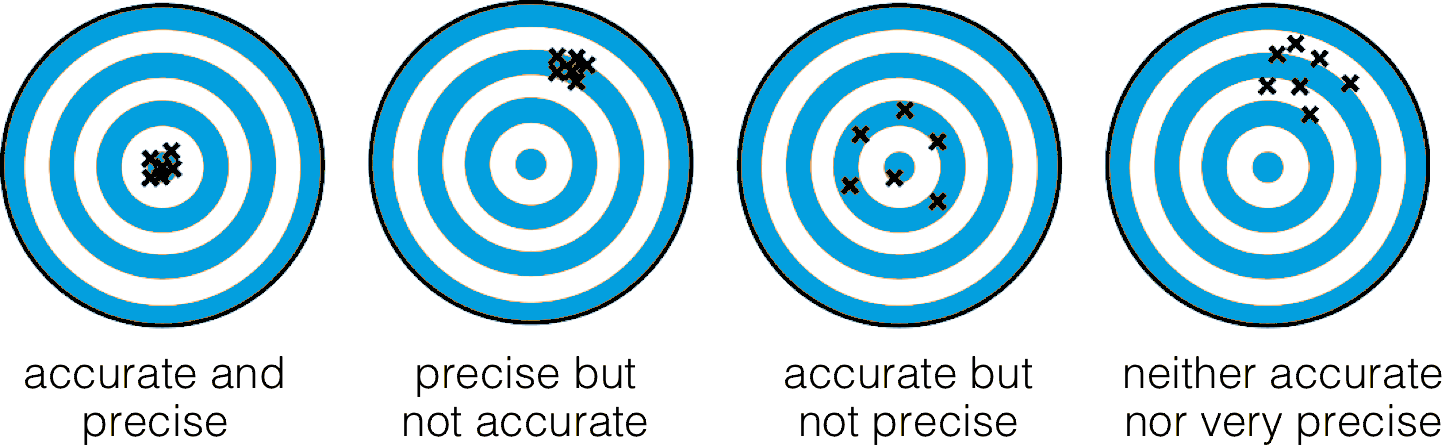
\includegraphics[width=\textwidth]{images/DP/targets.png}
\caption{\small Accuracy as bias, precision as standard errror.} \label{fig:targets}
\end{figure}
\afterpage{\FloatBarrier}
\item 
\textbf{consistency} -- are there conflicting observations (e.g. an individual has no children, but the age of one kid is recorded, etc.)?, and 
\item \textbf{uniformity} -- are units used uniformly throughout (e.g. an individual is 6ft tall, whereas another one is 145cm tall)?\end{itemize}
Finding an issue with data quality after the analyses are completed is a surefire way of losing the client's trust -- check early and often!
\paragraph{Common Sources of Error}
If the analysts have some control over the data collection and initial processing, regular data validation tests are easier to set-up. When the analysts are dealing with \textbf{legacy}, \textbf{inherited}, or \textbf{combined} datasets, it can be difficult to recognise errors arising (among others) from \begin{itemize}[noitemsep] \item missing data being given a code; \item `NA`/`blank' entries being given a code; \item data entry errors;\item coding errors;\item measurement errors;\item duplicate entries, and \item heaping (see Figure~\ref{fig:heaping} for an example).\end{itemize} 
\begin{figure}[t]
\centering
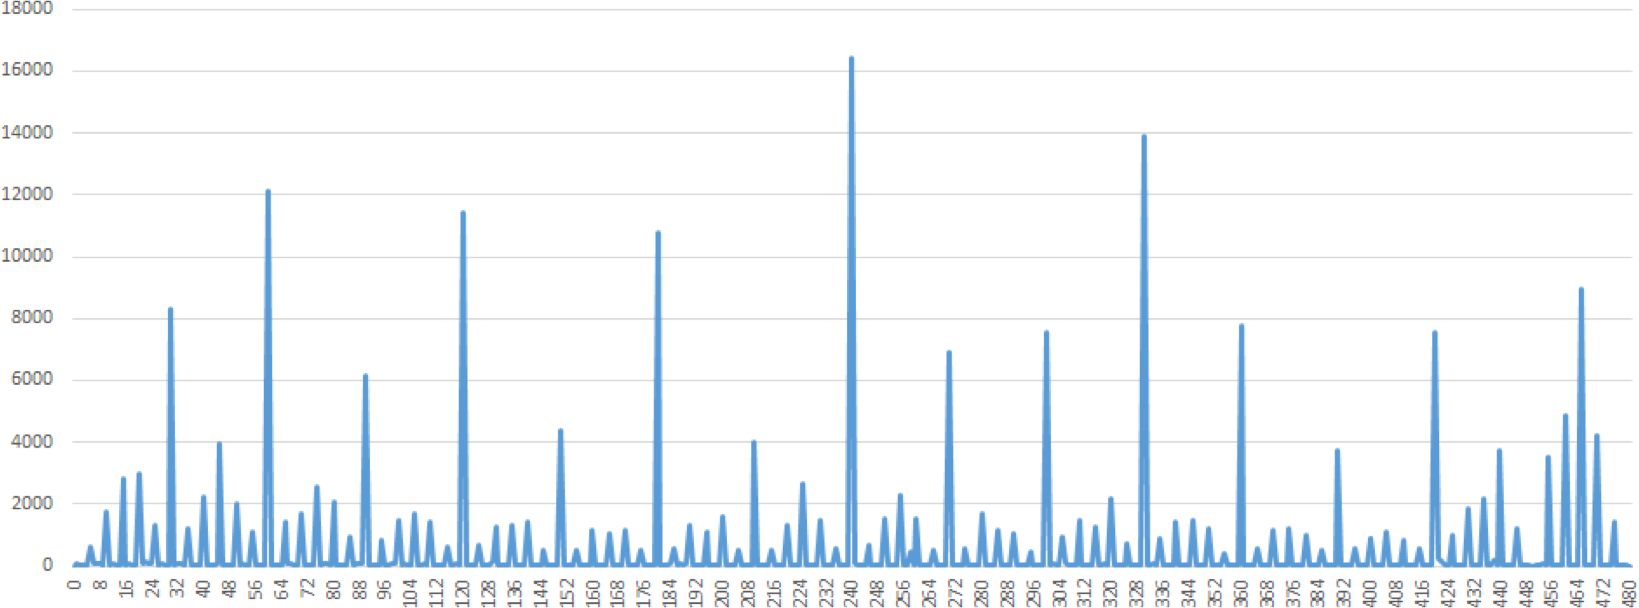
\includegraphics[width=\textwidth]{images/DP/heaping.png}
\caption[\small An illustration of heaping]{\small An illustration of heaping: self-reported time spent working in a day (personal file). Note the rounding off at various multiples of 5 minutes.} \hrule \label{fig:heaping}
\end{figure}
\afterpage{\FloatBarrier}
\paragraph{Detecting Invalid Entries}
Potentially invalid entries can be detected with the help of a number of methods: 
\begin{itemize}[noitemsep]
    \item \textbf{univariate descriptive statistics} -- count, range, $z-$score, mean, median, standard deviation, logic check, etc.;
    \item \textbf{multivariate descriptive statistics} -- $n-$way tables and logic check, and \item \textbf{data visualisation} -- scatterplot, histogram, joint histogram, etc.
\end{itemize} 
We will briefly discuss these methods in Sections~\ref{sec:SA} and \ref{sec:DV}. For now, we simply point out that univariate tests do not always tell the whole story. 
\begin{center}
    \rule{0.5\textwidth}{.4pt}
\end{center}
Consider, for instance, a medical dataset consisting of 38 patients' records, containing, among others, fields for the \textbf{sex} and the \textbf{pregnancy status} of the patients. A summary of the data of interest is afforded by the frequency counts (1-way tables) shown in Table~\ref{tab:1way}.
\begin{table}[t]
       \centering
        \begin{subtable}[b]{0.40\textwidth}
                \centering
                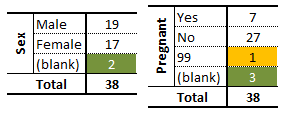
\includegraphics[width=\textwidth]{images/DP/med_sex_preg}
                \caption{\small 1-way tables} \label{tab:1way}
        \end{subtable}
        \begin{subtable}[b]{0.40\textwidth}
                \centering
                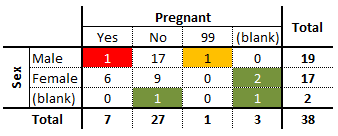
\includegraphics[width=\textwidth]{images/DP/med_2_way}
                \caption{\small 2-way table} \label{tab:2way}
        \end{subtable}
        \caption{\small Summary data for an (artificial) medical dataset.}\hrule
        \label{tab:med_data}
\end{table}

The analyst can quickly notice that some values are missing (in green) and that an entry has been miscoded as 99 (in yellow). Using only these univariate summaries, however, it is impossible to decide what to do with these invalid entries.\newpage\noindent The 2-way frequency counts of Table~\ref{tab:2way} shed some light on the situation, and uncover other potential issues with the data. One of the green entries is actually blank along the two variables; depending on the other information, this entry could be a candidate for \textbf{imputation} or outright \textbf{deletion} (more on these concepts in the next section). Three other observations are missing a value along exactly one variable, but the information provided by the other variables may be complete enough to warrant imputation. Of course, if more information is available about the patients, the analyst may be able to determine why the values were missing in the first place, although privacy concerns at the collection stage might muddy the waters. The miscoded information on the pregnancy status is linked to a male client, and as such re-coding it as `No' is likely to be a reasonable decision (although not necessarily the correct one). A similar reasoning process might make the analyst question the validity of the entry shaded in red -- the entry might very well be correct, but it is important to at the very least inquire about this data point, as this could lead to an eventual re-framing of the definitions and questions used at the collection stage.   
\begin{center}
    \rule{0.5\textwidth}{.4pt}
\end{center}
In general, there is no universal or one-size-fits-all approach -- a lot depends on the \textbf{nature of the data}. As always, domain expertise can help. Remember that a failure to detect invalid entries is \textbf{not a guarantee} that there are in fact no invalid entries in the dataset. It is important not to oversell this step to the client. When only a small number of invalid entries are detected, the general recommendation is to treat these values as  \textbf{missing}, which we discuss presently.
\subsubsection{Missing Values}    
\begin{tcolorbox}[title=Easier Said Than Done]
Obviously, the best way to treat missing data is not to have any. \\[-0.6cm]
\begin{flushright}
-- T. Orchard, M. Woodbury, \textit{A Missing Information Principle: Theory and Applications}, 1972
\end{flushright}
\end{tcolorbox}
\noindent Why does it matter that some values may be \textbf{missing}? On top of potentially introducing bias into the analysis, most analytical methods can not easily accommodate missing observations. Consequently, when faced with missing observations, analysts have two options: they can either \textbf{discard} the missing observation (which is not typically recommended, unless the data is missing completely randomly), or they can \textbf{create a replacement value} for the missing observation (the \textbf{imputation} strategy has drawbacks since we can never be certain that the replacement value is the true value, but is often the best available option; information in this section is taken partly from \cite{DP_Shinnie,DP_RLVHS,DP_vB,DP_R}).
\newpage\noindent Blank fields come in 4 flavours: \begin{itemize}[noitemsep]\item \textbf{nonresponse} -- an observation was expected but none was entered; \item  \textbf{data entry issues} -- an observation was recorded but was not entered in the dataset; \item \textbf{invalid entries} -- an observation was recorded but was considered invalid and has been removed, and \item  \textbf{expected blanks} -- a field has been left blank, but not unexpectedly so.
\end{itemize}
Too many missing values of the first three types can be indicative of \textbf{issues with the data collection process}, while too many missing values of the fourth type can be indicative of \textbf{poor questionnaire design} (see Section~\ref{sec:DC} for a brief discussion on these topics). Either way, missing values cannot simply be \textbf{ignored}.
\paragraph{Missing Value Mechanisms} The relevance of an imputation method is dependent on the underlying \textbf{missing value mechanism}; values may be 
\begin{itemize}[noitemsep]
\item \textbf{missing completely at random} (MCAR) -- the item absence is independent of its value or of the unit's auxiliary variables (e.g., an electrical surge randomly deletes an observation in the dataset); 
\item \textbf{missing at random} (MAR) -- the item absence is not completely random, and could, in theory, be accounted by the unit's complete auxiliary information, if available (e.g., if women are less likely to tell you their age than men for societal reasons, but not because of the age values  themselves), and 
\item \textbf{not missing at random} (NMAR) -- the reason for nonresponse is related to the item value (e.g., if illicit drug users are less likely to admit to drug use than teetotalers).
\end{itemize}
The consultant's main challenge in that regard is that the missing mechanism cannot typically be determined with any degree of certainty.
\paragraph{Imputation Methods}
There are numerous statistical \textbf{imputation} methods. They each have their strengths and weaknesses; consequently, consultants should take care to select a method which is appropriate for the situation at hand. They work best under MCAR or MAR, but they all tend to produce \textbf{biased estimates}.
\begin{figure}[t]
\centering
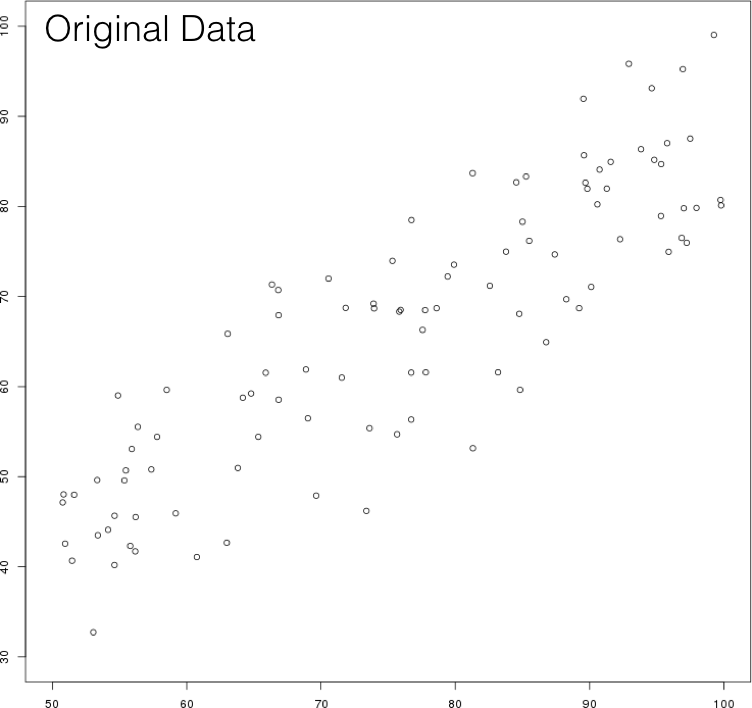
\includegraphics[width=0.4\textwidth]{images/DP/original.png}
\caption[\small Dr. Vanderwhede's original \textit{Advanced Retroencabulation} dataset]{\small Dr. Vanderwhede's original \textit{Advanced Retroencabulation} dataset; mid-term grades on the $x-$axis, final exam grades on the $y-$axis.} \label{fig:ori}\hrule
\end{figure}
\afterpage{\FloatBarrier}
\begin{itemize}[noitemsep]
\item In \textbf{list-wise deletion}, all units with at least one missing value are removed from the dataset. This straightforward imputation strategy assumes MCAR, but it can introduce bias if MCAR does not hold, and it leads to a reduction in the sample size and an increase in standard errors.
\item In \textbf{mean} or \textbf{most frequent imputation}, the missing values are substituted by the average or most frequent value in the unit's subpopulation group (stratum). This approach also assumes MCAR is commonly used, but it can creates distortions in the underlying distributions (such as a spike at the mean) and create spurious relationships among variables.
\item  In \textbf{regression} or \textbf{correlation imputation}, the missing values are substituted using a regression on the other variables. This model assumes MAR and trains the regression on units with complete information, in order to take full advantage of the auxiliary information when it is available. However, it artificially reduces data variability and produces over-estimates of correlations.
\item In \textbf{stochastic regression imputation}, the regression estimates are augmented with with random error terms added. Just as in the previous case, the model assumes MAR; an added benefit is that it tends to produce estimates that ``look'' more realistic than regression imputation, but it comes with an increased risk of type I error (false positives) due to small standard errors.
\item\textbf{Last observation carried forward} (LOCF) and its cousin \textbf{next observation carried backward} (NOCB) are useful for longitudinal data; a missing value can simply be substituted by the previous or next value. LOCF and NOCB can be used when the values do not vary greatly from one observation to the next, and when values are MCAR. Their main drawback is that they may be too ``generous'', depending on the nature of study. 
\item Finally, in \textbf{$k$-nearest-neighbour imputation}, a missing entry in a MAR scenario is substituted by the average (or median, or mode) value from the subgroup of the $k$ most similar complete respondents. This requires a notion of \textbf{similarity} between units (which is not always easy to define reasonably). The choice of $k$ is somewhat arbitrary and can affect the imputation, potentially distorting the data structure when it is too  large. 
\end{itemize}
\begin{center}
    \rule{0.5\textwidth}{.4pt}
\end{center}
\begin{figure}[t]
\centering
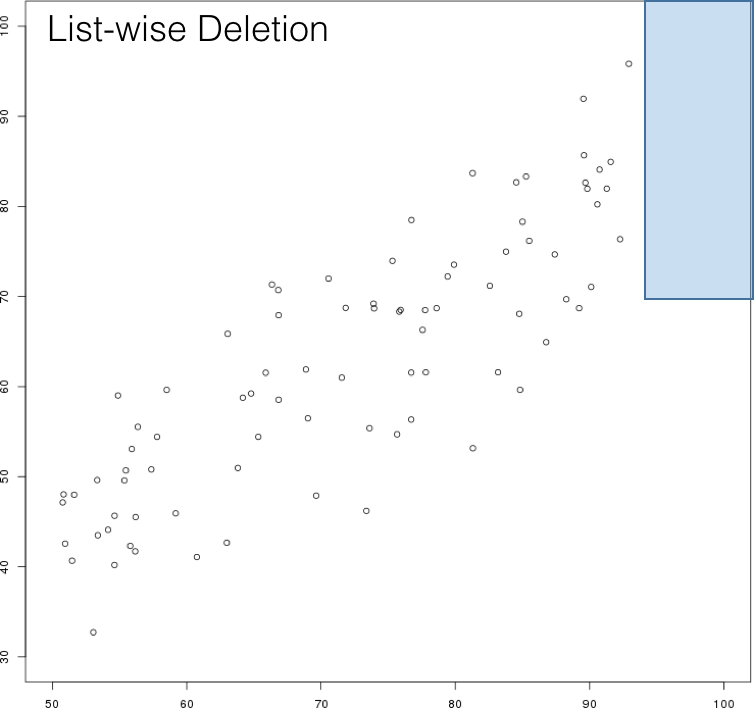
\includegraphics[width=0.4\textwidth]{images/DP/listwisedeletion.png}
\quad
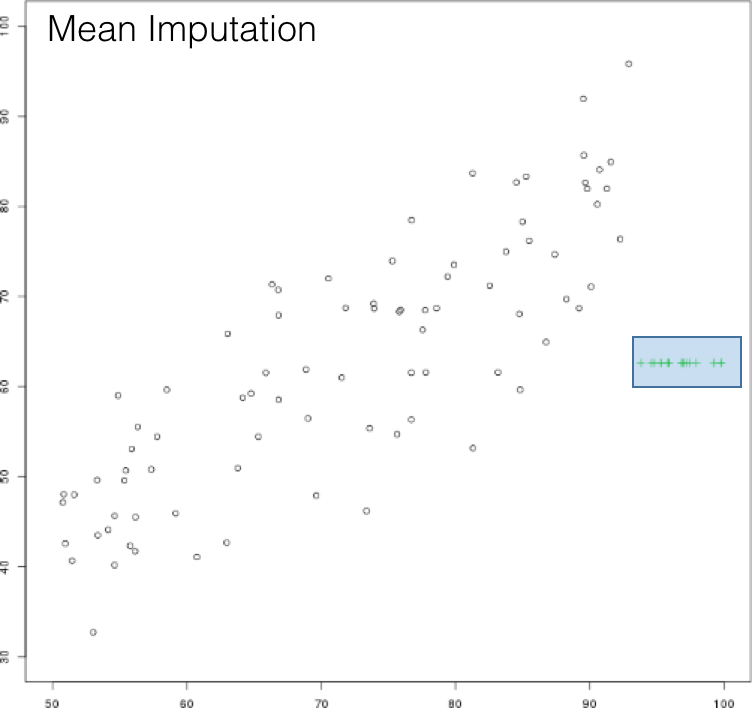
\includegraphics[width=0.4\textwidth]{images/DP/mean.png} \\
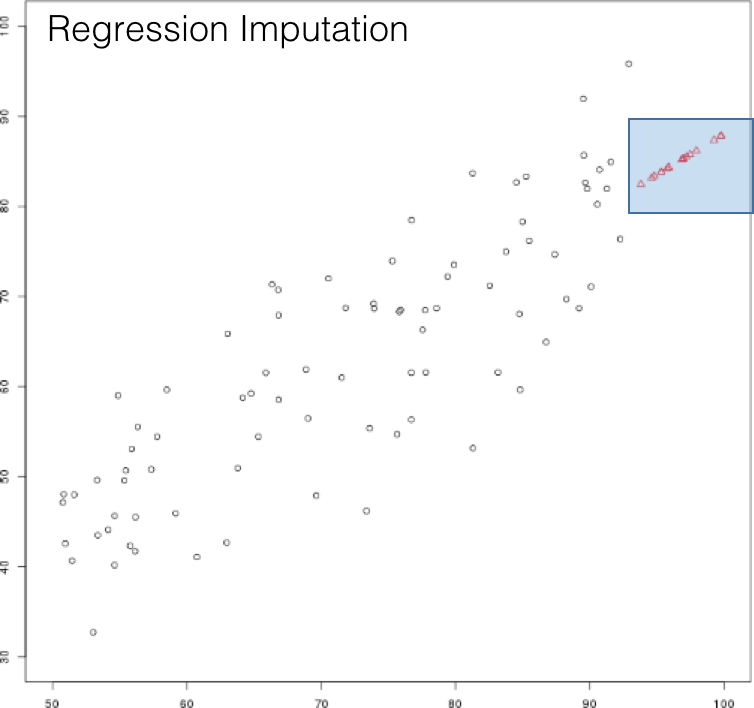
\includegraphics[width=0.4\textwidth]{images/DP/regression.png} 
\quad
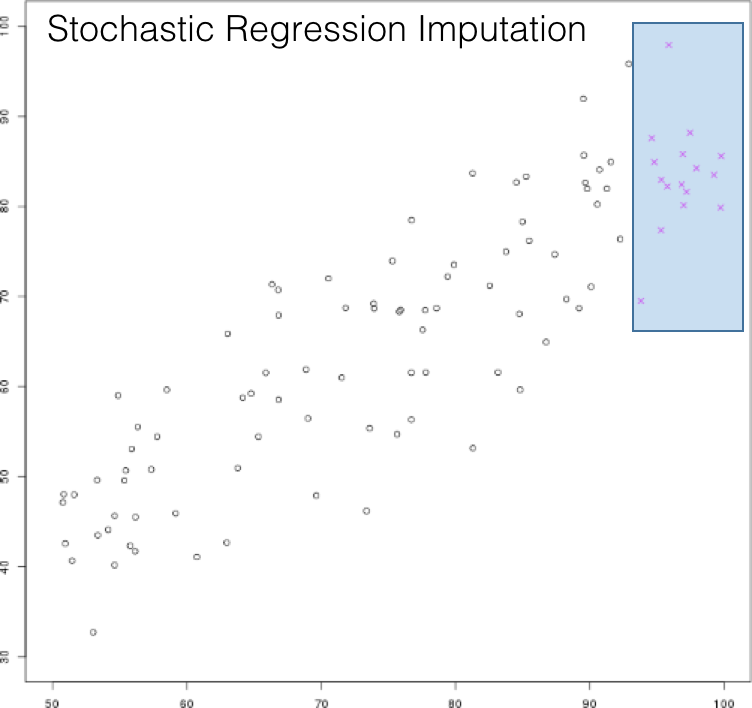
\includegraphics[width=0.4\textwidth]{images/DP/stochastic.png}
\caption[\small Imputed values for Dr. Vanderwhede's dataset]{\small Imputed values for Dr. Vanderwhede's dataset.}
\hrule\label{fig:theimputations}
\end{figure}
\afterpage{\FloatBarrier}
What would imputation look like in practice? Consider the following scenario (which is somewhat embarrassingly based on a real event). After marking the final exams of the 100 students who did not drop her course in \textit{Advanced Retroencabulation} at State University, Dr. Helga Vanderwhede plots the final exam grades ($y$) against the mid-term exam grades ($x$) as in Figure~\ref{fig:ori}. \par She takes a quick look at the data and sees that high final exam grades are \textbf{correlated} with high mid-term exam grades, and \textit{vice-versa}. She also sees that there is a fair amount of variability in the data: the noise is not very tight around the line of best fit. Furthermore, she realises that the final exam was harder than the students expected; she suspects that they just did not prepare for the exam seriously (and not that she made the exam too difficult, no matter what her ratings on \texttt{RateMyProfessor.com} suggest), as most of them could not match their mid-term exam performance. 
\newpage\noindent As Dr. Vanderwhede comes to term with her disappointment, she decides to take a deeper look at the numbers, at some point sorting the dataset according to the mid-term exam grades. It looks like good old Mary Sue performed better on the final than on the mid-term (where performance was already superlative), scoring the only perfect score. What a fantastic student Mary Sue is! And such a good person -- in spite of her superior intellect, she is adored by all of her classmates, thanks to her sunny disposition and willingness to help at all times. If only all students were like Mary Sue... She continues to toy with the spreadsheet, and the phone rings. After a long and exhausting conversation with Dean Bitterman about teaching loads and University's reputation, Dr. Vanderwhede returns to the spreadsheet and notices in horror that she has accidentally deleted the final exam grades of all students with a mid-term grade greater than 92. What is she to do? \par A technically-savvy consultant would advise her to either undo her changes or to close the file without saving the changes (or better yet, to re-enter the final grades by comparing with the physical papers), but let's assume for the time being that, in full panic mode, the only solution that comes to her mind is to impute the missing values. She knows that the missing final grades are MAR (and not MCAR since she remembers sorting the data along the $x$ values); she produces the imputations shown in Figure~\ref{fig:theimputations}. She remembers what the data looked like originally, and concludes that the best imputation method is the stochastic regression model.
\newpage\noindent
But this only applies to this specific example. In general, that might not be the case, however, due to various \textit{No Free Lunch} results (we will discuss this important technical results and its ramifications in Section~\ref{sec:DSML}). The principal take-away from this example is that various imputation strategies lead to different outcomes, and perhaps more importantly, that even though the imputed data might ``look'' like the true data, we have no way to measure its \textbf{departure from reality}. Any single imputed value is likely to be completely off. Mathematically, this might not be problematic, as the average departure might be relatively small, but in a business or personal context, this might create gigantic problems  -- how is Mary Sue likely to feel about Dr. Vanderwhede's solution in the previous example? How is Dean Bitterman likely to react, if he finds out about the imputation scenario from irrate students? Even though such questions are not quantitative in nature, they will have an effect on actionable solutions.  
\paragraph{Multiple Imputation}
Another drawback of imputation is that it tends to increase the noise in the data, because the imputed data is treated as the \textit{actual} data. In \textbf{multiple imputation}, the impact of that noise can be reduced by consolidating the analysis outcome from multiple imputed datasets. Once an imputation strategy has been selected on the basis of the (assumed) missing value mechanism, 
\begin{enumerate}[noitemsep]
\item the imputation process is repeated $m$ times to produce $m$ versions of the dataset;
\item each of these datasets is analyzed, yielding $m$ outcomes, and  
\item the $m$ outcomes are pooled into a single result for which the mean, variance, and confidence intervals are known.
\end{enumerate}
On the plus side, multiple imputation is \textbf{easy to implement}, \textbf{flexible}, as it can  be used in a most situations (MCAR, MAR, even NMAR in certain cases), and it accounts for \textbf{uncertainty} in the imputed values. However, $m$ may need to be quite \textbf{large} when the values are missing in large quantities from many of the dataset's features, which can substantially slow down the analyses. There may also be additional technical challenges when the output of the analyses is not a single value but some more complicated object.

\subsubsection{Anomalous Observations}
\begin{tcolorbox}[title=The Good Doctor's Take]
The most exciting phrase to hear [...], the one that heralds the most discoveries, is not ``Eureka!'' but ``That's funny...''.
 \\[-0.6cm]
\begin{flushright}
-- Isaac Asimov (attributed) 
\end{flushright}
\end{tcolorbox}
\noindent
\textbf{Outlying observations} are data points which are \textbf{atypical} in comparison to the unit's remaining features (\textit{within-unit}), or in comparison to the measurements for other units (\textit{between-units}), or as part of a collective subset of observations. Outliers are thus observations which are \textbf{dissimilar to other cases} or which contradict \textbf{known dependencies} or rules. Outlying observations may be anomalous along any of the individual variables, or in combination (information in this section is taken partly from \cite{DP_OW,DP_A,DP_T,DP_CBK}).
\newl Consider, for instance, an adult male who is 6-foot tall. Such a man would fall in the 86th percentile in Canada \cite{DP_HPC}, which, while on the tall side is not unusual; but in Bolivia, he would fall in the 99.9th percentile \cite{DP_HPC}, which would mark him as extremely tall and quite dissimilar to the rest of the population. (Why is there such a large discrepancy in the two populations?)  
\begin{center}
    \rule{0.5\textwidth}{.4pt}
\end{center}
The most common mistake that analysts make when dealing with outlying observations is to remove them from the dataset without careful studying whether there are good reasons to retain them. \newl \textbf{Influential data points}, meanwhile, are observations whose absence leads to \textbf{markedly different} analysis results. When influential observations are identified, remedial measures (such as data transformation strategies) may need to be applied to minimize any undue effect. Note that outliers may be influential, and influential data points may be outliers, but the conditions are neither necessary nor sufficient. 
\paragraph{Detecting Anomalies}  Anomalies are by definition \textbf{infrequent}, and typically shrouded in \textbf{uncertainty} due to small (relative) sample sizes, which makes differentiating them from \textbf{noise} or \textbf{data entry errors} difficult. It could also be the case that the boundaries between a normal unit and a deviating unit is \textbf{fuzzy}; with the advent of e-shops, a purchase made at 3am local time does not necessarily ring alarm bells anymore. It is hard enough as it is to try to identify ``honest'' anomalies; when anomalies are associated with \textbf{malicious activities}, they are typically \textbf{disguised} to look like a normal observation, which muddies the picture even more. 
\newl
Numerous methods exist to identify anomalous observations; \textbf{none of them are foolproof} and judgement must be used. Methods that employ graphical aids (such as box-plots, scatterplots, scatterplot matrices, and 2D tours, for outliers, say \ref{sec:DV}) are particularly easy to implement and interpret, especially in a low-dimensional setting. Analytical methods also exist (using Cooke's or Mahalanobis' distances, say), but in general some additional level of analysis must be performed, especially when trying to identify influential points (\textit{cf.} \textbf{leverage}). 
\newl We do not recommend the general use of \textbf{automated detection/removal} -- as tempting as this might get when the dataset is large. This stems partly from the fact that that once the ``anomalous'' observations have been removed from the data set, previously ``regular'' observations can become anomalous in turn in the smaller dataset; it is not clear when the runaway train will stop.  \newl 
In the early stages, \textbf{simple data analyses} (such as descriptive statistics, 1- and 2-way tables, and  traditional visualisations) may be performed to help identify anomalous observations, or to obtain insights about the data, which could eventually lead to modifications of the analysis plan.
\paragraph{Outlier Tests} So how do we \textit{actually} detect outliers? Most methods come in one of two flavours: \textbf{supervised} and \textbf{unsupervised} (we will discuss those concepts -- and others -- in Section~\ref{sec:DSML}).\newl 
Supervised methods use a historical record of \textbf{labeled} (that is to say, previously identified) anomalous observations to build a \textbf{predictive classification or regression model} which estimates the probability that a unit is anomalous; domain expertise is required to tag the data. Since anomalies are typically \textbf{infrequent}, these models often have to accommodate the rare occurrence problem (more on this in Section~\ref{sec:DSML}). Unsupervised methods, on the other hand, use no previous information or data; the following traditional methods and tests of outlier detection fall into this category (note that \textbf{normality} of the underlying data is an assumption for most tests; how robust these tests are against departures from this assumption depends on the situation).
\begin{center}
    \rule{0.5\textwidth}{.4pt}
\end{center}
Perhaps the most commonly known such test is \textbf{Tukey's boxplot test}: for normally distributed data, regular observations typically lie between the \textbf{inner fences} $$Q_1-1.5(Q_3-Q_1) \quad\mbox{and}\quad Q_3+1.5(Q_3-Q_1).$$ \textbf{Suspected outliers} lie between the inner fences and the \textbf{outer fences} 
$$Q_1-1.5(Q_3-Q_1) \quad\mbox{and}\quad Q_3+1.5(Q_3-Q_1).$$
Points beyond the outer fences are identified as \textbf{outliers} ($Q_1$ and $Q_3$ represent the data's   $1^{\textrm{st}}$ and $3^{\textrm{rd}}$ quartile, respectively; see Figure~\ref{fig:boxplot}).
\begin{figure}[t]
\centering
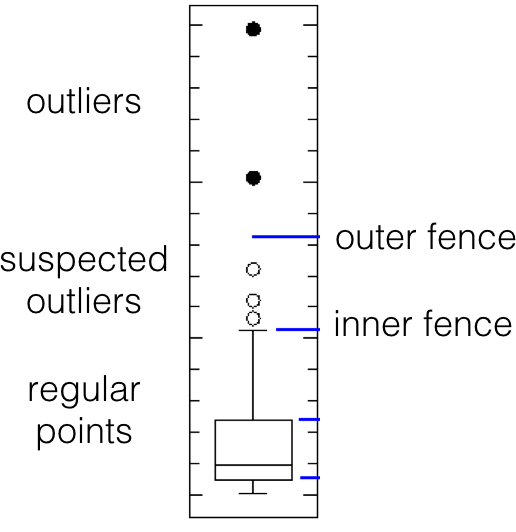
\includegraphics[width=0.30\textwidth]{images/DP/boxplot.png}
\caption[\small Tukey's boxplot test for outliers]{\small Tukey's boxplot test; suspected outliers are marked by white disks, outliers by black disks.}
\hrule\label{fig:boxplot}
\end{figure}
\afterpage{\FloatBarrier}
The \textbf{Grubbs test} is another univariate test, which takes into consideration the number of observations in the dataset. Let $x_i$ be the value of feature $X$ for the $i^{\textrm{th}}$ unit, $1\leq i\leq N$, $(\overline{x},s_x)$ be the mean and standard deviation of feature $X$, $\alpha$ be the significance level, and $T(\alpha,N)$ be the critical value of the Student $t$-distribution at significance $\alpha/2N$. Then, the $i^{\textrm{th}}$ unit is an \textbf{outlier along feature} $X$ if $$|x_i-\overline{x}| \geq \frac{s_x(N-1)}{\sqrt{N}}\sqrt{\frac{T^2(\alpha,N)}{N-2+T^2(\alpha,N)}}.$$
Other common tests include:
\begin{itemize}[noitemsep]
\item the \textbf{Dixon $Q$ test}, which is used in the experimental sciences to find outliers in (extremely) small datasets -- it is of dubious validity;
\item the \textbf{Mahalanobis distance}, which is linked to the leverage of an observation (a measure of influence), can also be used to find multi-dimensional outliers, when all relationships are linear (or nearly linear);
\item the \textbf{Tietjen-Moore} test, which is used to find a specific number of outliers;
\item the \textbf{generalized extreme studentized deviate}, if the number of outliers is unknown; 
\item the \textbf{chi-square} test, when outliers affect the foodneess-of-fit, as well as 
\item DBSCAN and other unsupervised outlier detection methods.
\end{itemize}
What do we do when the data is not normally distributed? We will discuss one possible approach after we present three more examples illustrating the basics of visual outlier and anomaly detection. 
\begin{center}
    \rule{0.5\textwidth}{.4pt}
\end{center}
On a specific day, the height of several plants in a nursery are measured. The records also show each plant's age (the number of days since the seed has been planted).    
\begin{figure}[t]
       \centering
        \begin{subfigure}[b]{0.30\textwidth}
                \centering
                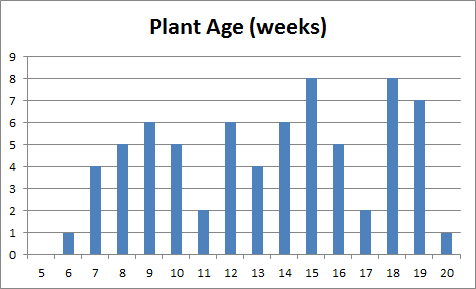
\includegraphics[width=\textwidth]{images/DP/plant_age}
                \caption{\small Age distribution}\label{fig:planta}
        \end{subfigure}
        \begin{subfigure}[b]{0.30\textwidth}
                \centering
                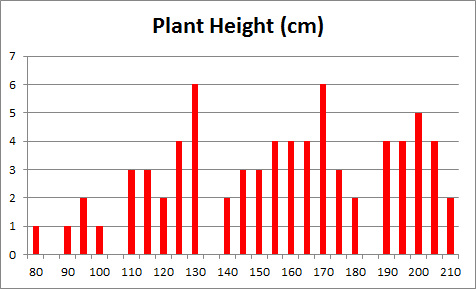
\includegraphics[width=\textwidth]{images/DP/plant_height}
                \caption{\small Height distribution}\label{fig:plantb} 
        \end{subfigure}
        \begin{subfigure}[b]{0.30\textwidth}
                \centering
                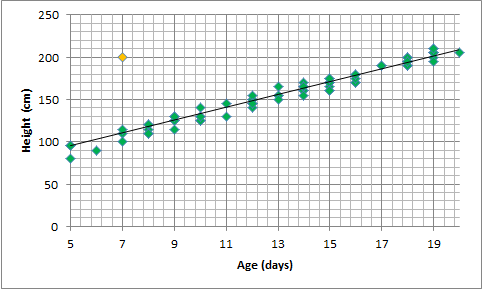
\includegraphics[width=\textwidth]{images/DP/plant_height_vs_age}
                \caption{\small Height vs age, with trend}\label{fig:plantc} 
        \end{subfigure}
        \caption[\small Summary visualisations for a plant dataset]{\small Summary visualisations for an (artificial) plant dataset.}
        \label{fig:plant_data}
\end{figure}
Histograms of the data are shown in Figures~\ref{fig:planta} and \ref{fig:plantb}. Very little can be said about the data at that stage: the age of the plants (controlled by the nursery staff) seems to be somewhat haphazard, as does the response variable (height). A scatter plot of the data (see Figure~\ref{fig:plantc}), however, reveals that growth is strongly correlated with age during the early days of a plant's life for the observations in the dataset; most points clutter around a linear trend. But one point (in yellow) is easily identified as an \textbf{outlier}. There are at least two possibilities: either that measurement was botched or mis-entered in the database (representing an invalid entry), or that one specimen has experienced unusual growth (outlier). Either way, the analyst has to investigate further.  
\begin{center}
    \rule{0.5\textwidth}{.4pt}
\end{center}
A government department has 11 service points in a jurisdiction. Service statistics are recorded: in particular, the monthly average arrival rates per teller and monthly average service rates per teller for each service point are available. A scatter plot of the service rate per teller ($y$ axis) against the arrival rate per teller ($x$ axis), with linear regression trend, is shown in Figure~\ref{fig:servicea}. The trend is seen to inch upwards with increasing $x$ values. A similar graph, but with the left-most point removed from consideration, is shown in Figure~\ref{fig:serviceb}. The trend still slopes upward, but the fit is significantly improved suggesting that the removed observation is unduly \textbf{influential} -- a better understanding of the relationship between arrivals and services is afforded if it is set aside. Any attempt to fit that data point into the model must take that information into consideration. Note, however, that influential observations depend on the analysis that is ultimately being conducted -- a point may be influential for one analysis, but not for another.     
\begin{figure}[t]
       \centering
        \begin{subfigure}[b]{0.30\textwidth}
                \centering
                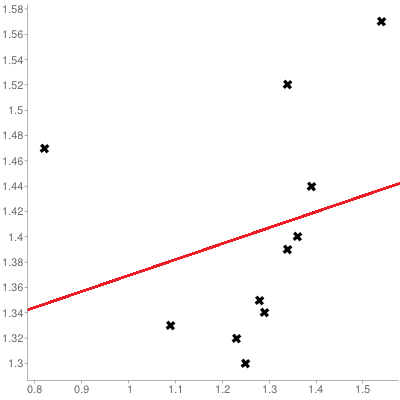
\includegraphics[width=\textwidth]{images/DP/scatter_plot_linear_1}
                \caption{\small Trend for 11 service points}
                \label{fig:servicea}
        \end{subfigure}
        \begin{subfigure}[b]{0.30\textwidth}
                \centering
                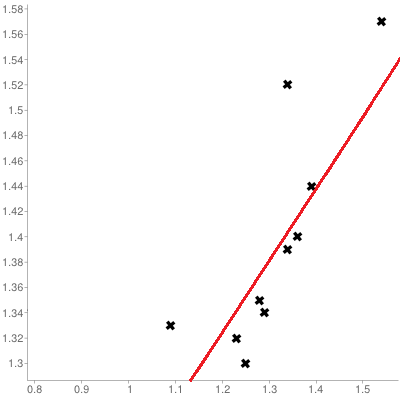
\includegraphics[width=\textwidth]{images/DP/scatter_plot_linear_2}
                \caption{\small Trend for 10 service points} \label{fig:serviceb}
        \end{subfigure}
        \begin{subfigure}[b]{0.30\textwidth}
                \centering
                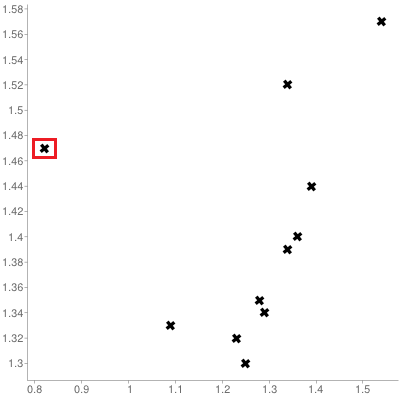
\includegraphics[width=\textwidth]{images/DP/scatter_plot_2}
                \caption{\small Influential observation}\label{fig:servicec} 
        \end{subfigure}
        \caption[\small Visualisations for a service point dataset]{\small Visualisations for an (artificial) service point dataset.}\hrule
        \label{fig:service_data}
\end{figure}
\begin{center}
    \rule{0.5\textwidth}{.4pt}
\end{center}
Measurements of the length of the appendage of a certain species of insect have been made on 71 individuals. Descriptive statistics have been computed; the results are shown in Figure~\ref{tab:appendagea}.
\begin{table}[t]
\centering
        \begin{subtable}[b]{0.26\textwidth}
                \centering
                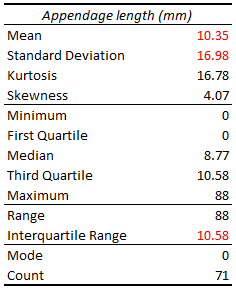
\includegraphics[width=\textwidth]{{images/DP/appendage_length_descriptive}}
                \caption{\small Descriptive statistics}\label{tab:appendagea}
        \end{subtable}
        \begin{subtable}[b]{0.50\textwidth}
                \centering
                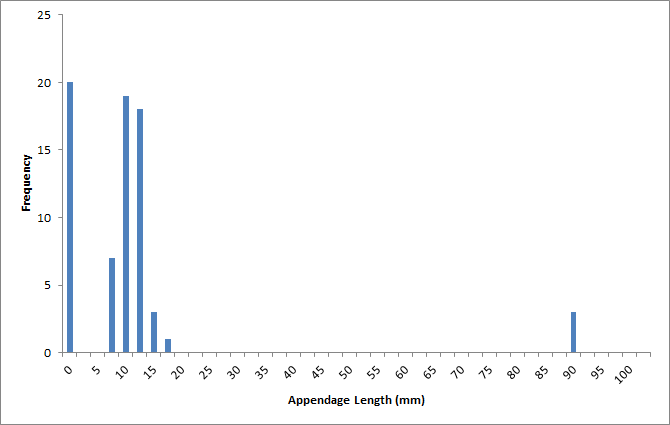
\includegraphics[width=\textwidth]{{images/DP/appendage_length}}
                \caption{\small Appendage length distribution}\label{tab:appendageb}
        \end{subtable}
\caption[\small Summary and visualisation for an appendage length dataset]{\small Summary and visualisation for an (artificial) appendage length dataset.}\hrule
\label{tab:appendage_data}
\end{table}
Analysts who are well-versed in statistical methods would recognise the tell-tale signs that the distribution of appendage lengths is likely to be asymmetrical (since the skewness is non-negligible) and to have a ``fat'' tail (due to the kurtosis being commensurate with the mean and the standard deviation, the range being so much larger than the interquartile range, and the maximum value being so much larger than the third quartile). The mode, minimum, and first quartile values belong to individuals without appendages, so there would appear to be two sub-groups in the population (perhaps split along the lines of juveniles/adults, or males/females). The maximum value has already been seen to be quite large compared to the rest of the observations, which at first suggests that it might belong to an \textbf{outlier} or \textbf{invalid entry}. The histogram of the measurements, however, shows that there are 3 individuals with very long appendages (see Figure~\ref{tab:appendageb}): it now becomes plausible for these anomalous entries to belong to individuals from a different species altogether who were \textbf{erroneously added} to the dataset. This does not, of course, constitute a proof of such an error, but it raises the possibility, which is often the best that a consultant can do for a client.   
\subsubsection{Data Transformation}
\begin{tcolorbox}[title=It's Also True of Data]
History is the transformation of tumultuous conquerors into silent footnotes. \\[-0.6cm]
\begin{flushright}
-- Paul Eldridge, American educator
\end{flushright}
\end{tcolorbox}
\noindent
This \textbf{crucial} last step is often neglected or omitted altogether when consultants embark on complex data analysis projects. Various transformation methods are available, depending on the analysts' needs and data types, including: \begin{itemize}[noitemsep]
\item \textbf{standardization} and \textbf{unit conversion}, which put the dataset's variables on an equal footing -- a requirement for basic comparison tasks and more complicated problems of clustering and similarity matching;
\item \textbf{normalization}, which  attempts to force a variable into a normal distribution -- an assumption which must be met in order to use a number of traditional analysis methods, such as regression analysis or ANOVA, and 
\item \textbf{smoothing methods}, which help remove unwanted noise from the data, but at a price -- perhps removing natural variance in the data. 
\end{itemize}
Another type of data transformation is pre-occupied with the concept of \textbf{dimensionality reduction}. There are many advantages to working with low-dimensional data:
\begin{itemize}[noitemsep]
\item \textbf{visualisation methods} of all kinds are available to extract and present insights out of such data (see Section~\ref{sec:DV});
\item high-dimensional datasets are subject to the so-called \textbf{curse of dimensionality}, which asserts (among other things) that multi-dimensional spaces are vast, and when the number of features
in a model increases, the number of observations required to maintain predictive
power also increases, but at a \textbf{substantially higher rate} (see Figure~\ref{fig:COD});
\item another consequence of the curse is that in high-dimension sets, all observations are roughly \textbf{dissimilar} to one another -- observations tend to be nearer the dataset's boundaries than they are to one another.  
\end{itemize}
\begin{figure}[t]
\centering
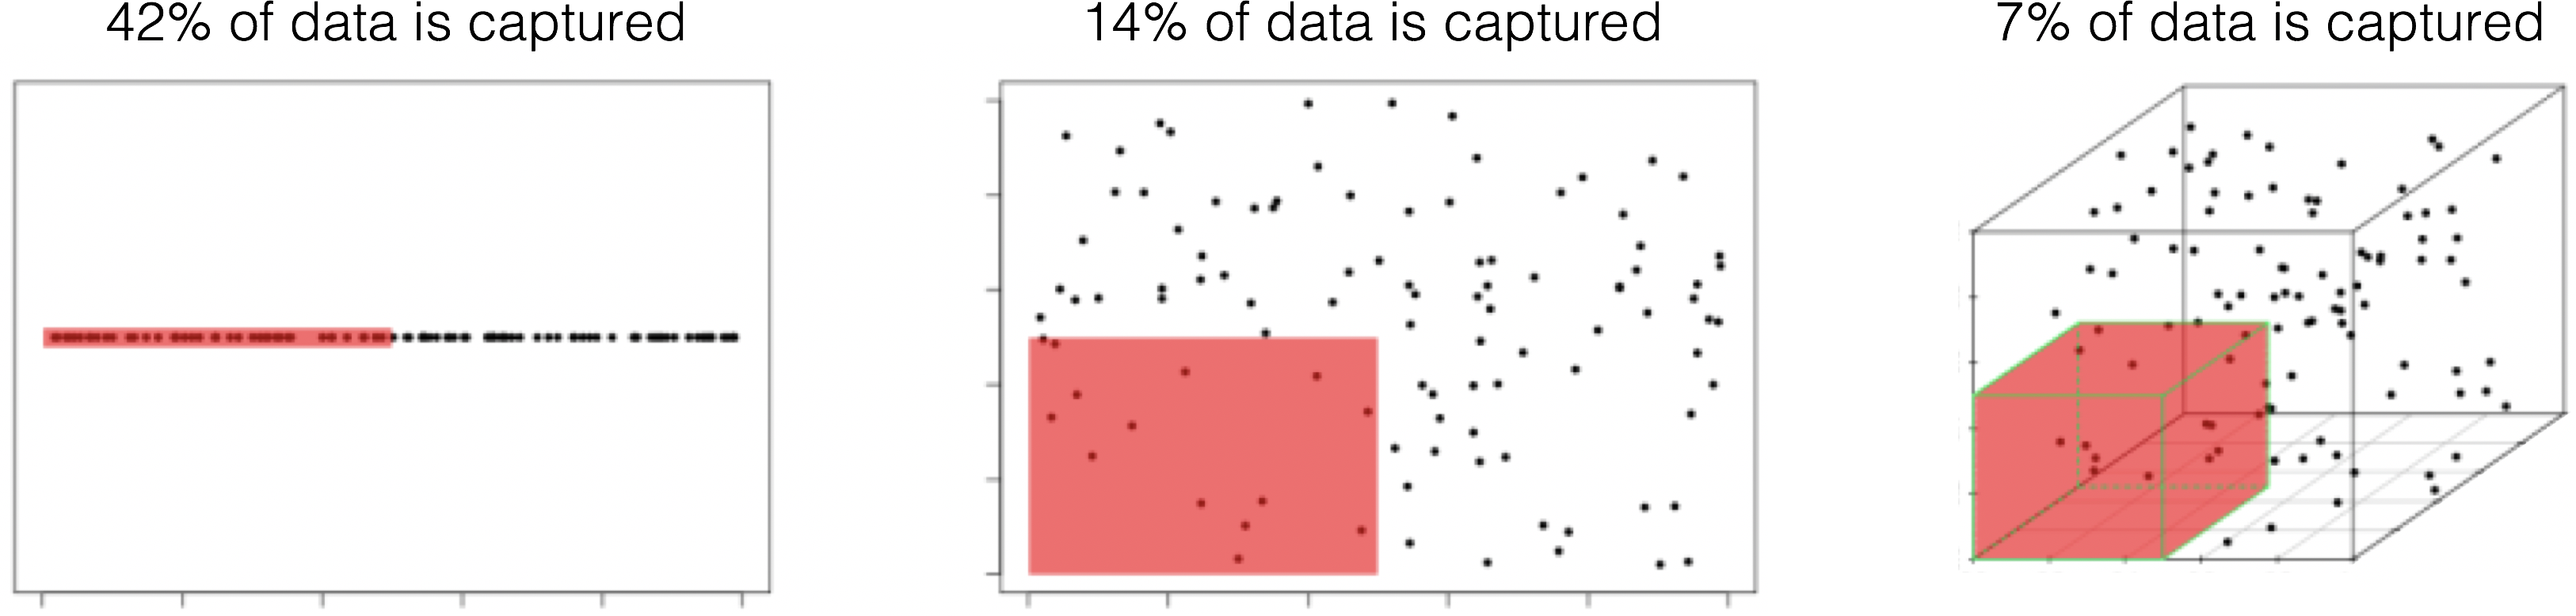
\includegraphics[width=\textwidth]{images/DP/COD.png}\caption[\small Illustration of the curse of dimensionality]{\small Illustration of the curse of dimensionality; $N=100$ observations are uniformly distributed on the unit hypercube $[0,1]^d$, $d=1, 2, 3$. The red regions represent the smaller hypercubes $[0,0.5]^d$, $d=1,2,3$. The percentage of captured datapoints is seen to decrease with an increase in $d$ \cite{DP_SS}.} \label{fig:COD}\hrule
\end{figure}
\afterpage{\FloatBarrier}
Dimension reduction techniques such as the ubiqituous \textbf{principal component analysis}, \textbf{independent component analysis}, and \textbf{factor analysis} (for numerical data), or \textbf{multiple correspondence analysis} (for categorical data) project multi-dimensional datasets onto low-dimensional but high-information spaces (the so-called \textbf{Manifold Hypothesis}). Some information is necessarily lost in the process, but in many instances the drain can be kept under control and the gains made by working with smaller datasets can offset the losses of completeness. We will touch on this topic briefly in Section~\ref{sec:DSML}.
\paragraph{Common Transformations} Models often require that certain data assumptions be met. For instance, ordinary least square regression assumes:
\begin{itemize}[noitemsep]
\item that the response variable is a \textbf{linear combination} of the predictors;
\item \textbf{constant} error variance; 
\item \textbf{uncorrelated residuals}, which may or may not be statistically independent;
\item etc.
\end{itemize}
In reality, it is rare that raw data  meets the requirements, but that does not necessarily mean that we need to abandon the model -- an \textbf{invertible} sequence of data transformations may produce a derived data set which \textit{does} meet the requirements, allowing the consultant to draw conclusions about the original data. \par In the regression context, invertibility is guaranteed by \textbf{monotonic} transformations:  identity, logarithmic, square root, inverse (all members of the power transformations), exponential, etc. (illustrations are provided in Figure~\ref{fig:transforms}).
\begin{figure}[t]
\centering
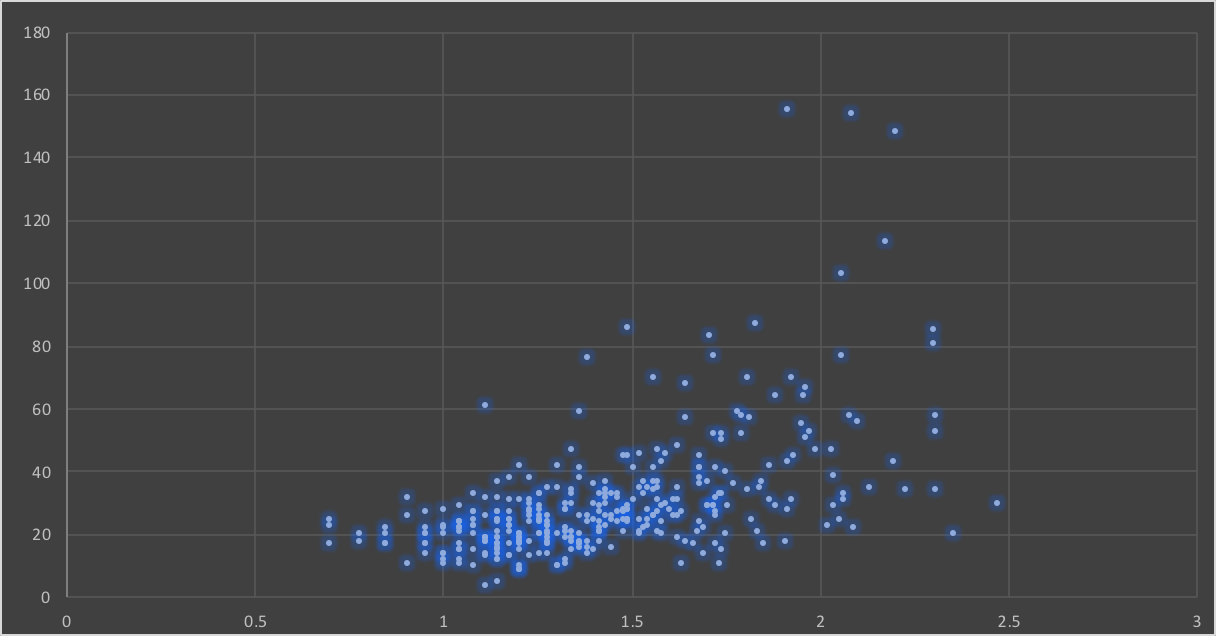
\includegraphics[width=0.45\textwidth]{images/DP/original_BUPA.png}
\quad
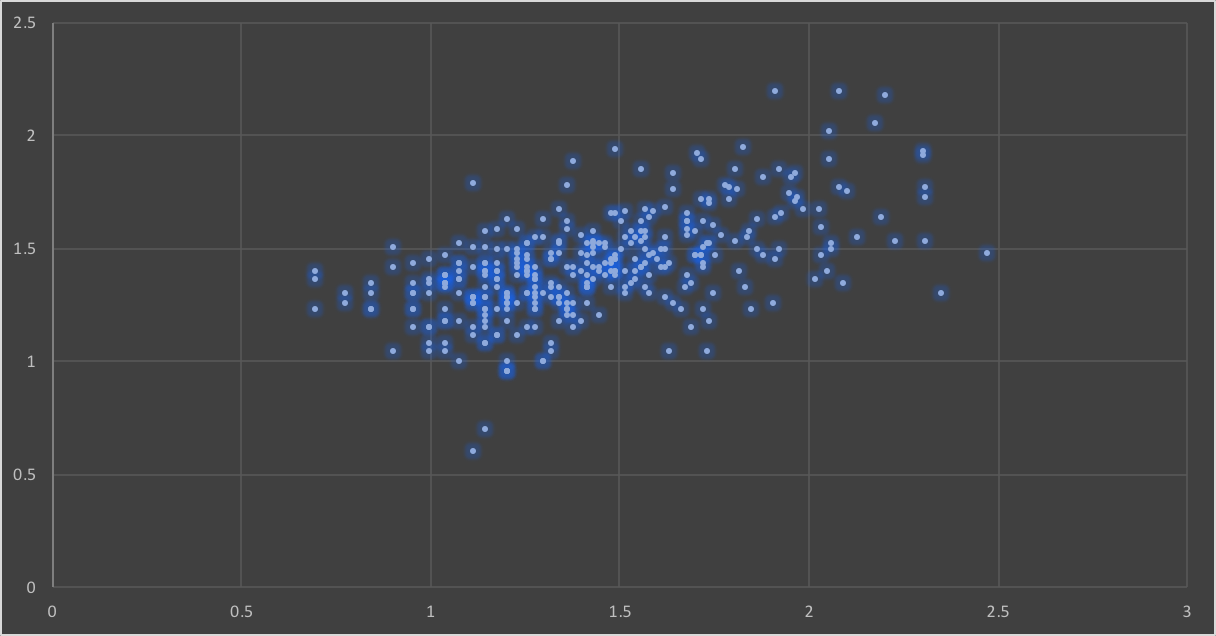
\includegraphics[width=0.45\textwidth]{images/DP/log.png} \\
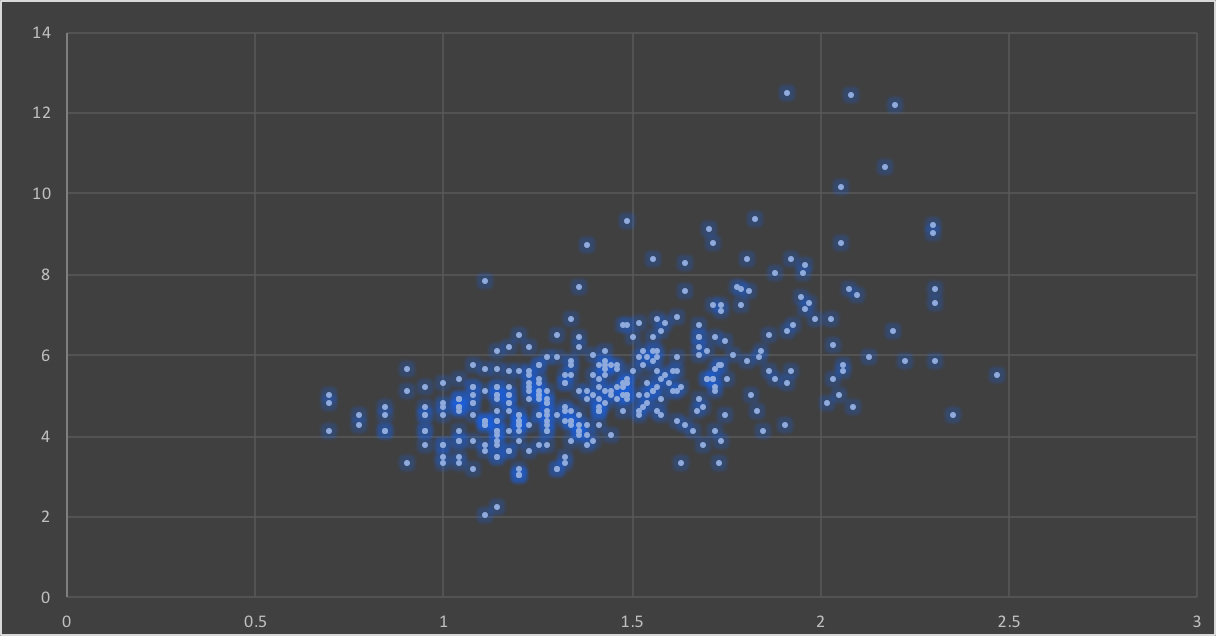
\includegraphics[width=0.45\textwidth]{images/DP/sqrt.png} 
\quad
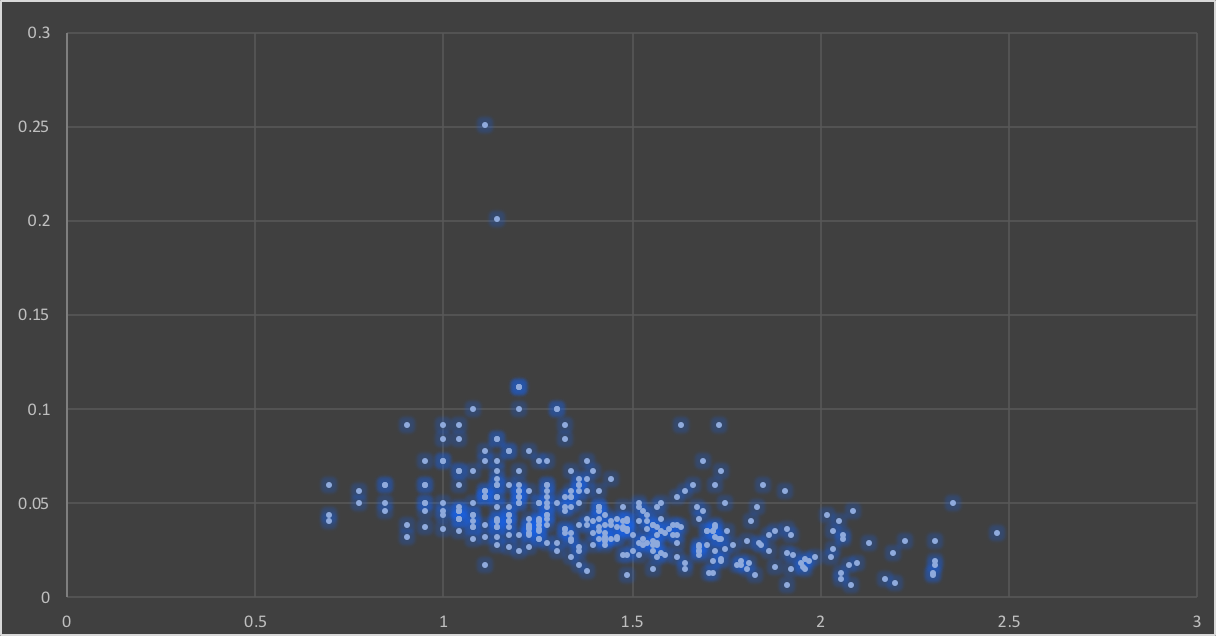
\includegraphics[width=0.45\textwidth]{images/DP/inverse.png} \\
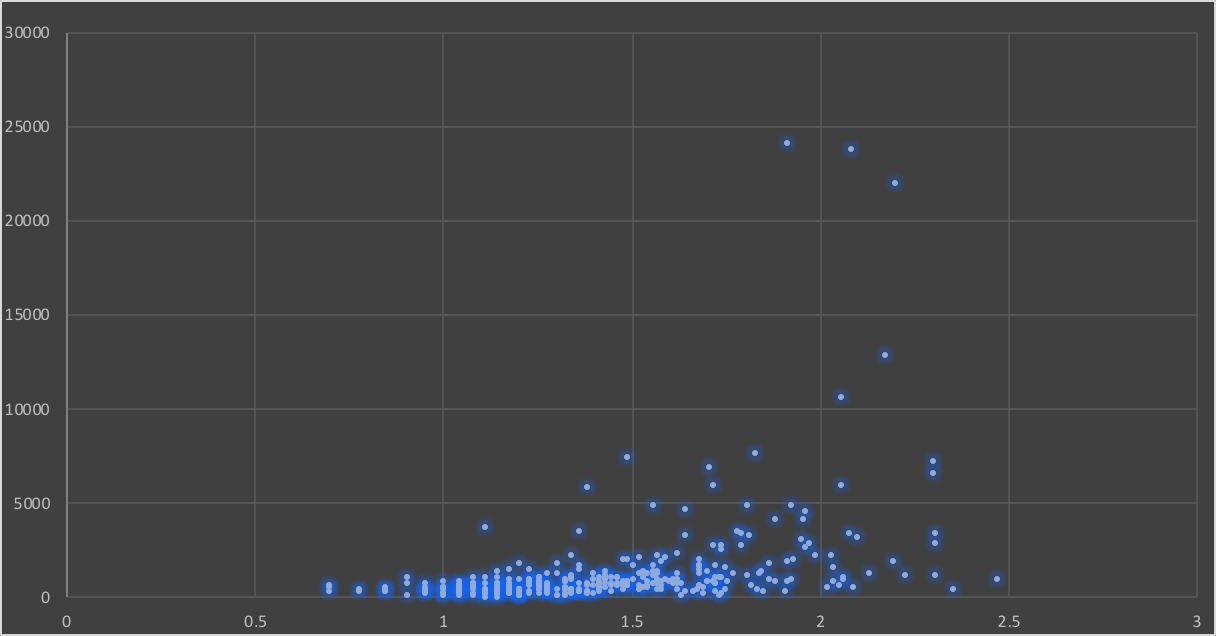
\includegraphics[width=0.45\textwidth]{images/DP/square.png} 
\quad
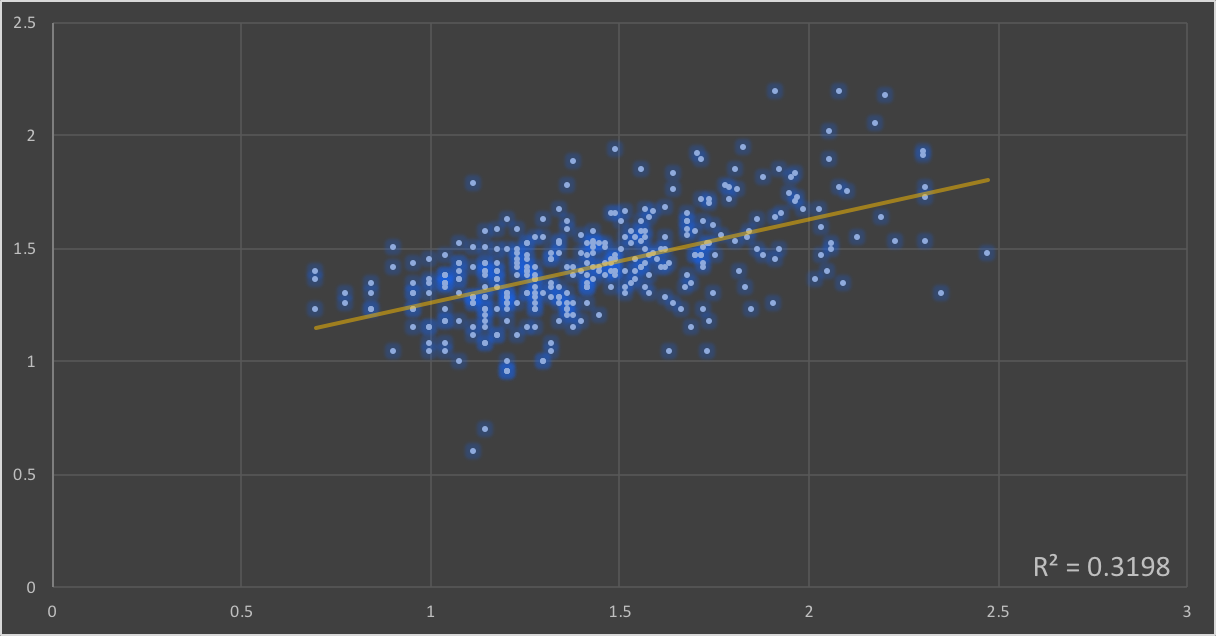
\includegraphics[width=0.45\textwidth]{images/DP/boxcox.png}
\caption[\small Examples of data transformations]{\small Examples of data transformations, for a subset of the BUPA liver dataset \cite{DP_BUPA}. From left to right, top to bottom: original data, $Y'=\log Y$, $Y'=\sqrt{Y}$, $Y'=\frac{1}{Y}$, $Y'=Y^2$, and Box-Cox best choice ($\approx$ log). }
\hrule\label{fig:transforms}
\end{figure}
\afterpage{\FloatBarrier}
There are rules of thumb and best practices to transform data, but consultants should not discount the importance of explore the data visually before making a choice. \newl Transformations on the predictors $X$ may be used to achieve the \textbf{linearity assumption}, but they usually come at a price -- correlations are not preserved by such transformations, for instance. Transformations on the target $Y$ can help with \textbf{non-normality} of residuals and \textbf{non-constant variance} of error terms. Note that transformations can be applied \textbf{both} to the target variable or the predictors: as an example, if the linear relationship between two variables $X$ and $Y$ is expressed as $Y=a+bX$, then a unit increase in $X$ is associated with an average of $b$ units in $Y$. But a better fit might be afforded by either of $$\log Y = a+bX,\quad Y=a+b\log X,\quad \mbox{or}\quad  \log Y = a+b\log X,$$ for which:
\begin{itemize}[noitemsep]
\item a unit increase in $X$ is associated with an average $b\%$ increase in $Y$;
\item a $1\%$ increase in $X$ is associated with an average $0.01b$ unit increase in $Y$, and
\item a $1\%$ increase in $X$ is associated with a $b\%$ increase in $Y$, respectively. 
\end{itemize}
\paragraph{Box-Cox Transformation} The choice of transformation is often as much of an art as it is a science. There is a common  framework, however, that provides the  optimal transformation, in a sense. Consider the task of predicting the target $Y$ with the help of the predictors $X_j$, $j=1,\ldots, p$. The usual model takes the form $$y_i=\sum_{j=1}^p\beta_jX_{x,i}+\varepsilon_i,\quad i=1,\ldots, n.$$ Perhaps the residuals are skewed, or their variance is not constant, or the trend itself does not appear to be linear. A power transformation might be preferable, but if so,  which one? \newl The \textbf{Box-Cox transformation} $y_i\mapsto y'_i(\lambda)$, $y_i>0$ is defined by  $$y'_i(\lambda)=\begin{cases}(y_1 \ldots   y_n)^{1/n}\ln y_i, \text{if }\lambda=0 \\ 
\frac{y_i^{\lambda}-1}{\lambda}(y_1 \ldots   y_n)^{\frac{1-\lambda}{n}}, \text{if }\lambda\neq 0
\end{cases};$$
variants allow for the inclusion of a shit parameter $\alpha>0$, which extends the transformation to $y_i>-\alpha$. The \textbf{suggested} choice of $\lambda$ is the value that maximises the log-likelihood $$\mathcal{L}=-\frac{n}{2}\log\left(\frac{2\pi\hat{\sigma}^2}{(y_1 \ldots   y_n)^{2(\lambda-1)/n}}+1\right).$$
There might be theoretical rationales which favour a particular choice of $\lambda$ -- these are not to be ignored. It is also important to produce a residual analysis, as the best Box-Cox choice does not necessarily meet all the least squares assumptions. Finally, it is important to remember that the resulting parameters have the least squares property \textbf{only with respect to the transformed data points}. 
\paragraph{Scaling} Numeric variables may have different scales (weights and heights, for instance). Since the variance of a large-range variable is typically greater than that of a small-range variable, leaving the data \textbf{unscaled} may introduce biases, especially when using unsupervised methods. It could also be the case that it is the relative positions/rankings which is of importance, in which case it could become important to look at relative distances between levels: 
\begin{itemize}[noitemsep]
\item \textbf{standardisation} creates a variable with mean 0 and standard deviations 1: $$Y_i=\frac{X_i-\overline{X}}{s_X};$$
\item \textbf{normalization} creates a new variable in the range [0,1]: $$Y_i=\frac{X_i-\min {X}}{\max X- \min X}.$$
\end{itemize}
These are not the only options. Different schemes canlead to different outputs. 
\paragraph{Discretising} To reduce computational complexity, a numeric variable may need to be replaced with an \textbf{ordinal} variable (\textit{height} values could be replaced by the qualitative ``\textit{short}'', ``\textit{average}'', and ``\textit{tall}'', for instance. Of course, what these terms represent depend on the context: Canadian short and Bolivian tall may be fairly commensurate.  It is far from obvious how to  determine the bins' limits  -- \textbf{domain expertise} can help, but it could introduce unconscious bias to the analyses. In the absence of such expertise, limits can be set so that either
\begin{itemize}[noitemsep]
\item the bins each contain the same \textbf{number of observations};
\item the bins each have the same \textbf{width}, or 
\item the performance of some modeling tool is maximised. 
\end{itemize}
Again, various choices may lead to different outputs. 
\paragraph{Creating Variables} Finally, it is possible that new variables may need to be introduced (in contrast with dimensionality reduction). These new variables may arise
\begin{itemize}[noitemsep]
\item as \textbf{functional relationships} of some subset of available features (introducing powers of a feature, or principal components, say);
\item because modeling tool may require \textbf{independence of observations} or \textbf{independence of features} (in order to remove multicolinearity, for instance), or 
\item to simplify the analysis by looking at \textbf{aggregated summaries} (often used in text analysis).
\end{itemize}
There is no limit to the number of new variables that can be added to a dataset -- but consultants should strive for \textbf{relevant additions}.
%\subsubsection{Case Study: Cleaning Ottawa Professional Fire Fighters Association Data}
\subsubsection{Case Study: Imputation of Blood Alcohol Content Levels}
When fatal collisions occur, it is frequently the case that at least one of the drivers (or one of the pedestrians/cyclists, as the case may be) involved in the collision was affected by alcohol. Since breathalyzer tests cannot be conducted on deceased individuals, the presence of alcohol in the blood cannot be confirmed until the coroner's report becomes available. 
\newl In large jurisdictions, distances to the coroner's office may take a while to traverse. A large volume of such fatalities may also slow down the process. For these (and other) reasons, it can take up to a year for the missing \textbf{blood alcohol concentration} (BAC) levels to make their way to various interested parties (policy makers, analysts, etc.). This can cause delays in policy implementation and could possibly lead to otherwise preventable deaths, data analysts often resort to imputation methods in order to make an \textbf{informed guess} as to the BAC level in fatal collisions. This prediction is made on the basis of a number of auxiliary variables, such as the age of the driver. Once the imputed values are supplanted by the coroner's values, BAC-dependent preliminary analyses with the imputed values can easily be re-conducted with the actual values to obtain up-to-date results.
\newl In 2007, \textit{Ministry of Transportation of Ontario} (MTO) faced such a situation: using a small number of features (many of which have missing values themselves), is it possible to 
\begin{enumerate}[noitemsep]
    \item predict whether alcohol was involved, and if so, 
    \item predict the BAC level?
\end{enumerate}
The problem is easily stated, but the existence of an actionable solution is not clear. There may simply be no link between the available features and the BAC level. For instance, how strong can the connection between the deceased's handedness and their BAC level (assuming we even have access to that information). \newl Another issue, which we have broached in Section~\ref{sec:DC}, is the question of the data's representativeness: is it possible that whatever link might have existed in 2007 is simply not going to be present in the future, perhaps as a result of implemented policies? If that is the case, how useful would a general model prove to be? 
\newl The paper that describes the two-stage multiple imputation model used by \textit{Transport Canada} to solve the MTO's problem is presented after the references -- note how the flow is broken when the tables are not labeled. 


\phantomsection
\begin{thebibliography}{99}
\bibitem{DP_C}
Chapman, A. [2005], Principles and Methods of Data Cleaning - Primary Species and Species-Occurrence Data, Report for the Global Biodiversity Information Facility, Copenhagen.
\bibitem{DP_vB}van Buuren, S. [2012], Flexible Imputation of Missing Data, CRC Press, Boca Raton.
\bibitem{DP_Shinnie}Hagiwara, S. [2012], Nonresponse Error in Survey Sampling - Comparison of Different Imputation Methods, Honours Thesis, Carleton University, Ottawa.
\bibitem{DP_RLVHS}Raghunathan, T., Lepkowski, J., Van Hoewyk, J. and Solenberger, P. [2001], A Multivariate Technique for Multiply Imputing Missing Values Using a Sequence of Regression Models, Survey Methodology, v.27, n.1, pp.85-95, Statistics Canada, Catalogue no. 12-001.
\bibitem{DP_R}Rubin, D.B. [1987], Multiple Imputation for Nonresponse in Surveys, Wiley, New York.
\bibitem{DP_KNNL}Kutner, M., Nachtsheim, C., Neter, J. and Li, W. [2004], Applied Linear Statistical Models, 5th ed., McGraw-Hill/Irwin, New York.
\bibitem{DP_GS}Green, S. and Salkind, N. [2011], Using SPSS for Windows and Macintosh - Analyzing and Understanding Data, 6th ed., Prentice Hall, Upper Saddle River.
\bibitem{DP_DC}Wikipedia entry for Data Cleansing 
\bibitem{DP_I}Wikipedia entry for Imputation
\bibitem{DP_O}Wikipedia entry for Outliers
\bibitem{DP_T}Torgo, L. [2017], Data Mining with R (2nd edition), CRC Press.
\bibitem{DP_M}McCallum, Q.E. [2013], Bad Data Handbook, O'Reilly.
\bibitem{DP_KJ}Kazil, J., Jarmul, K. [2016], Data Wrangling with Python, O'Reilly
\bibitem{DP_dJvdL}de Jonge, E., van der Loo, M. [2013], An Introduction to Data Cleaning with R, Statistics Netherlands.
\bibitem{DP_P}Pyle, D. [1999], Data Preparation for Data Mining, Morgan Kaufmann Publishers.
\bibitem{DP_WI}Weiss, S.M., Indurkhya, I. [1999], Predictive Data Mining: A Practical Guide, Morgan Kaufmann Publishers.
\bibitem{DP_B}Buttrey, S.E. [2017], A Data Scientist's Guide to Acquiring, Cleaning, and Managing Data in R, Wiley.
\bibitem{DP_A}Aggarwal, C.C. [2013], Outlier Analysis, Springer.
\bibitem{DP_CBK}Chandola, V., Banerjee, A., Kumar, V. [2007], Outlier detection: a survey, Technical Report TR 07-017, Department of Computer Science and Engineering, University of Minnesota.
\bibitem{DP_HA}Hodge, V., Austin, J. [2004], A survey of outlier detection methodologies, Artif.Intell.Rev., 22(2):85-126.
\bibitem{DP_FNWO}Feng, L., Nowak, G., Welsh, A.H., O'Neill, T. [2014], imputeR: a general imputation framework in R.
\bibitem{DP_S}Steiger, J.H. , Transformations to Linearity, lecture notes.
\bibitem{DP_W}Wood, F., Remedial Measures Wrap-Up and Transformations, lecture notes. 
\bibitem{DP_DKS}Dougherty, J., Kohavi, R., Sahami, M. [1995], Supervised and unsupervised discretization of continuous features, in Machine Learning: Proceedings of the Twelfth International Conference, Prieditis, A., Russell, S. (eds), Morgan Kaufmann Publishers. 
\bibitem{DP_OW}Orchard, T., Woodbury, M. [1972], A Missing Information Principle: Theory and Applications, Berkeley Symposium on Mathematical Statistics and Probability, University of California Press.  
\bibitem{DP_HPC}Height Percentile Calculator, by Age and Country, https://tall.life/height-percentile-calculator-age-country/ 
\bibitem{DP_BUPA} Dua, D., Karra Taniskidou, E. [2017], Liver Disorders dataset, UCI Machine Learning Repository.
\bibitem{DP_SS} https://simplystatistics.org/2014/10/24/an-interactive-visualization-to-teach-about-the-curse-of-dimensionality/ 
\end{thebibliography}
\setboolean{@twoside}{false}
\includepdf[pages={1-9},offset={50 -40}]{documents/BAC_jur.pdf}
\setboolean{@twoside}{true}
